\section{Initial CSI Data Gathering}
These are the results of gathering initial CSI data using Linux shell commands into a .dat file.
\begin{figure}[H]%
    \centering
    \subfloat[\lstinline{ping} gateway IP at 192.168.0.1]{{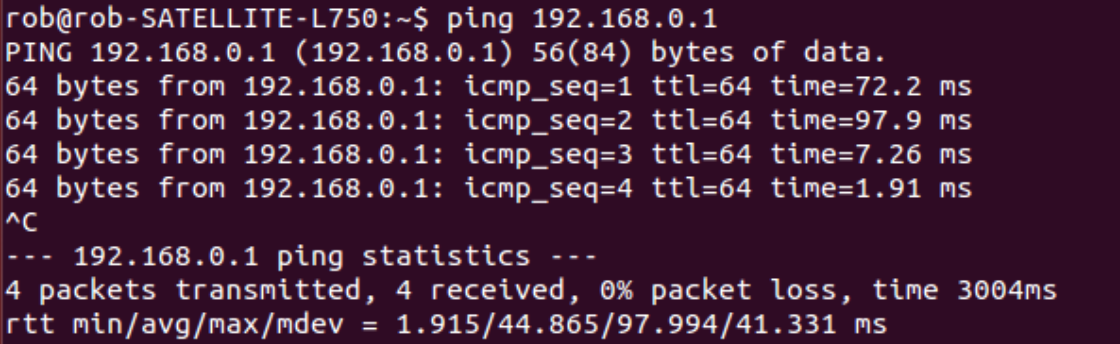
\includegraphics[width=7cm]{Figures/ping.png} }}%
    \qquad
    \subfloat[Receiving data using \lstinline{log_to_file}]{{\includegraphics[width=7cm]{Figures/Receiving.png} }}%
    \caption{Using \lstinline{ping} \& \lstinline{log_to_file} to send and receive ICMP packets between Archer C6 router and laptop}%
    \label{fig:UbuntuTerminals}%
\end{figure}
Hence, I was able to present one packet's SNR and CSI-phase across the 30 subcarriers once the data was converted to absolute units. Each stream conveys similar information as seen by each coloured trace. However, there isn't enough information to understand anything about the surrounding environment. 
\begin{figure}[H]%
    \centering
    \subfloat[CSI amplitude of each stream for one packet]{{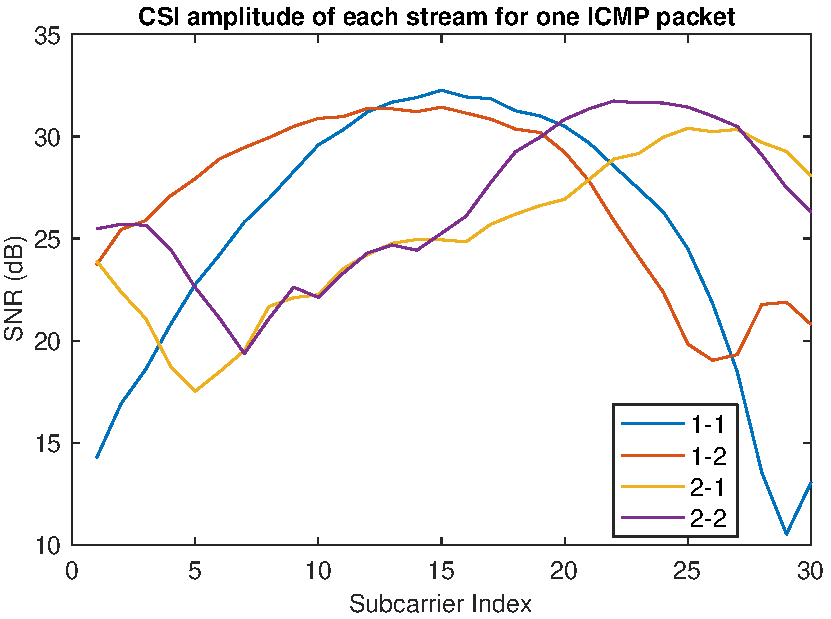
\includegraphics[scale = 0.5]{Figures/CSI_amplitude_subcarriers.pdf} }}%
    \qquad
    \subfloat[Wrapped phase of each stream for one packet]{{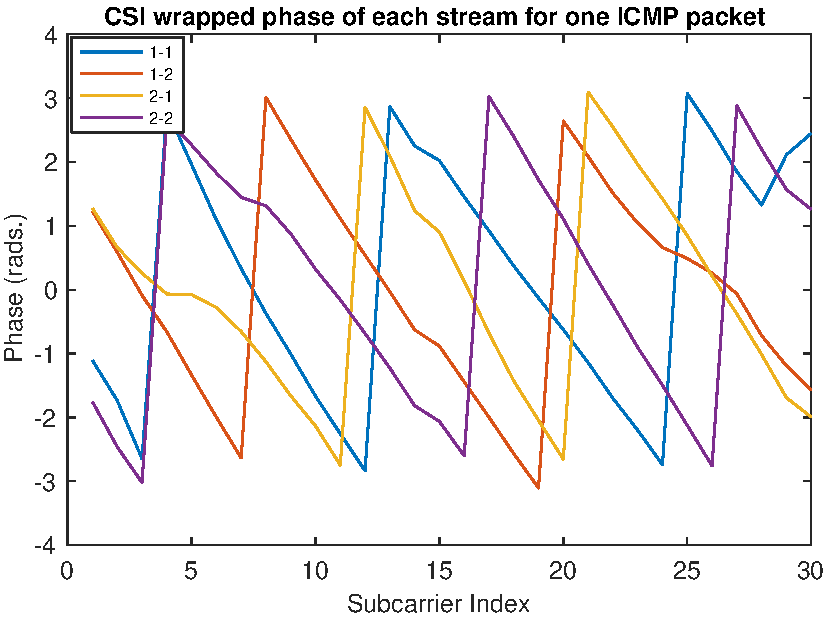
\includegraphics[width=7cm]{Figures/CSI_phase_subcarriers.pdf} }}%
    \caption{($2\times 2$ MIMO-OFDM system) CSI amplitude experiences frequency dependent fading at the edges of the channel bandwidth (Subcarriers 1 and 30). CSI phase is wrapped between $\pi$ and $-\pi$ rads. in a typical '$zig-zag$' pattern}%
    \label{fig:CSIAMPLITUDE&PHASE}%
\end{figure}
The CSI phase can be unwrapped using \lstinline{unwrap} in MATLAB to verify the phase according to RT-Fall and \cite{perceivingAccurateCSI}. It was decreasing for each consecutive subcarrier.
\begin{comment}\begin{figure}[H]
    \centering
  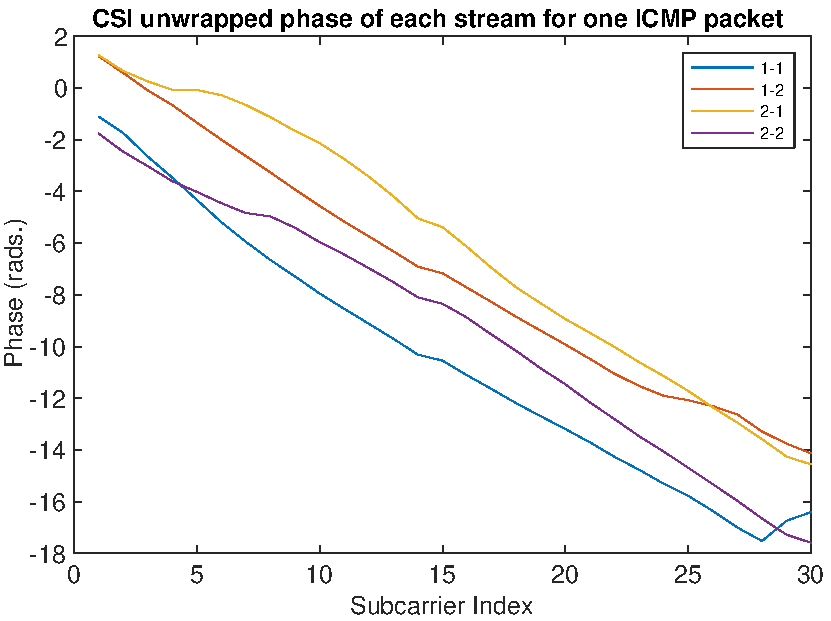
\includegraphics[scale=0.5]{Figures/CSI_unwrapped_subcarriers.pdf}
  \caption{CSI unwrapped phase for each of the 4 streams is presented correctly as descending for all 30 subcarriers}
  \label{fig:unwrappedPhase}
\end{figure}\end{comment}
However, each stream has 30 values per packet. A link between each of these needed to be found to simplify the calculations:
\begin{figure}[H]%
    \centering
    \subfloat[Different Streams for Subcarrier 15]{{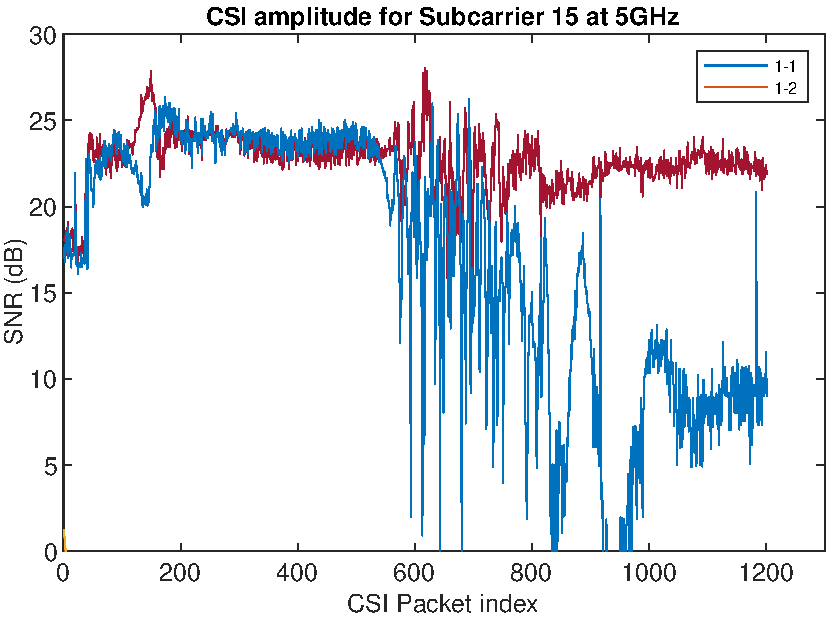
\includegraphics[scale = 0.5]{Figures/subcarrier15.pdf} }}%
    \qquad
    \subfloat[Different subcarriers in Stream 1-1]{{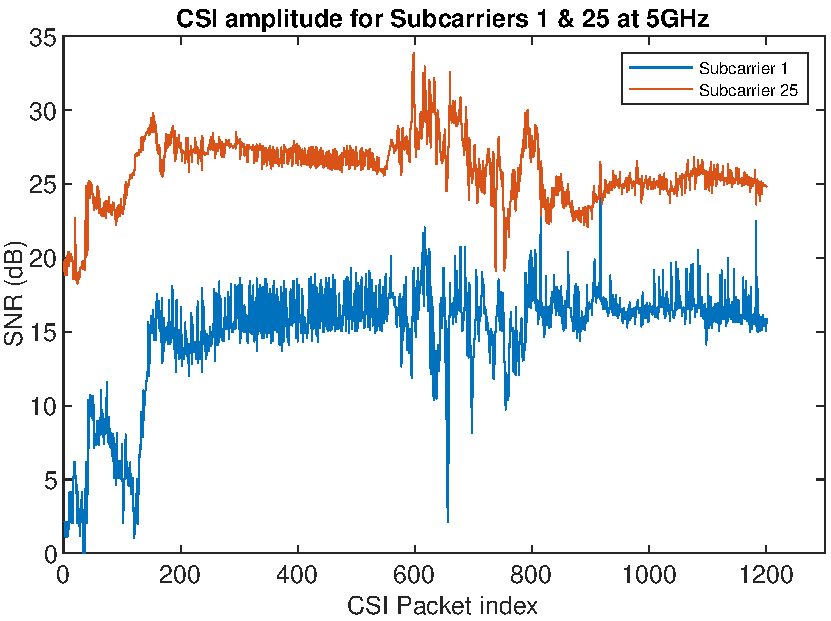
\includegraphics[scale=0.5]{Figures/differentSubcarriers.pdf} }}%
    \caption{Demonstrating that different streams react differently to human activity in (a) but different subcarriers in the same stream act similarly in (b)}%
    \label{fig:subcarriersVSstreams}%
\end{figure}
In Figure 4.4 (a), the fall occurring at the 600th packet affects streams 1-1, 1-2 differently due to the large change in the blue plot compared to red. However, human activities affect subcarriers similarly as seen in Figure 4.4 (b). This allows me to use the Equation \ref{eqn:3.1} to average the subcarriers into 1 value for each stream. 
\section{Data Processing}
\subsection{CSI Amplitude}
%%%%%%%%%%%%%%%%%%%%%%%%%%%%%%
The result of using Eqn. \ref{eqn:3.1} is shown below where the 30 subcarriers shown in Fig. 4.4 (a) are calculated and converted to one value per packet in Fig. 4.4 (b). The overall shape of the subcarriers is preserved but the full SNR range is not (some subcarriers have values around 27dB while Fig 4.5 (b)'s maximum point is 25dB). This implies a loss of frequency diversity in the calculation making it problematic for fall detection as seen by WiFall.
\begin{figure}[H]%
    \centering
    \subfloat[Subcarrier amplitudes in Stream 1-1]{{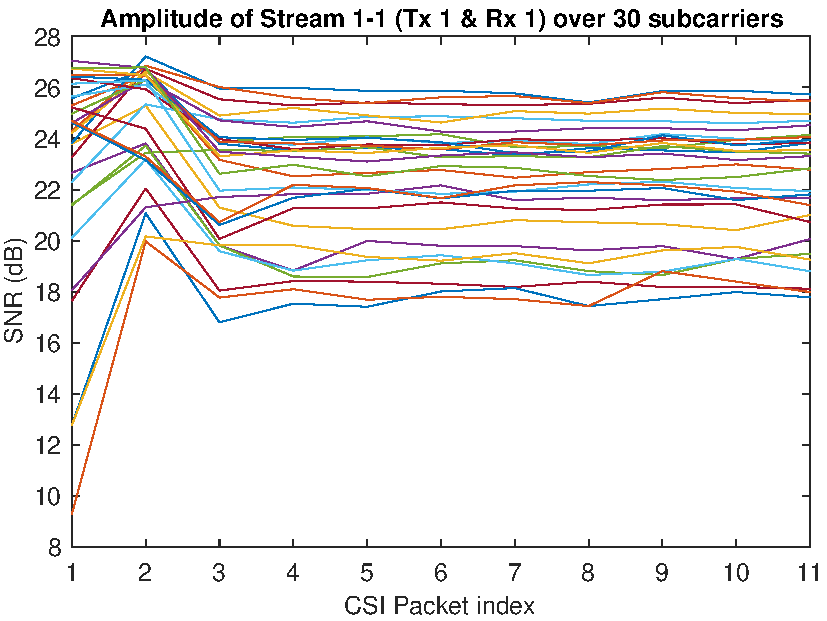
\includegraphics[scale = 0.5]{Figures/onlytaking10.pdf} }}%
    \qquad
    \subfloat[Averaged amplitude. One value per packet]{{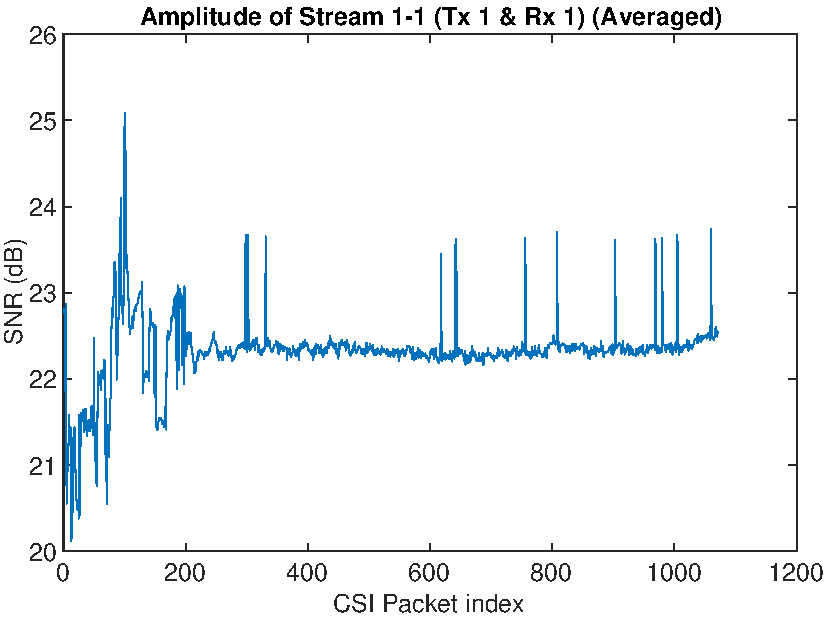
\includegraphics[scale=0.5]{Figures/averagedForAmplitude.pdf} }}%
    \caption{Using the findings from Fig. \ref{fig:subcarriersVSstreams}, I apply Eqn. \ref{eqn:3.1} to obtain a simpler plot in (b)}%
    \label{fig:applyingAmplitudeEquation}%
\end{figure}
\vspace{11pt}
\begin{figure}[H]
\centering
\begin{tabular}{cc}
  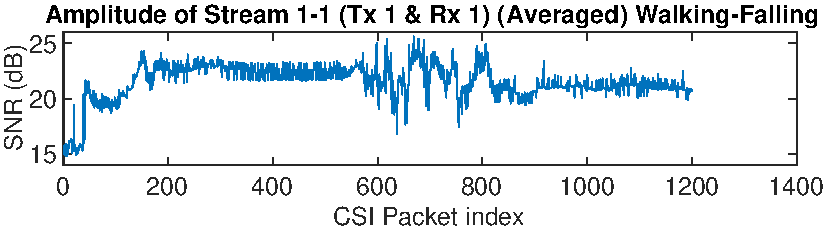
\includegraphics[scale = 0.5]{Figures/walkingFallingAveraged.pdf} &   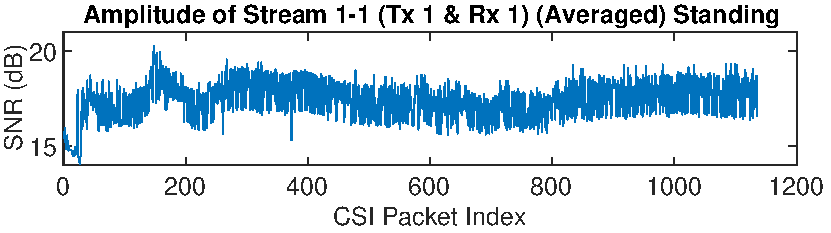
\includegraphics[scale=0.5]{Figures/standingForAmplitude.pdf} \\
(a) Person falling (600th packet) & (b) Person standing still \\[6pt]
\multicolumn{2}{c}{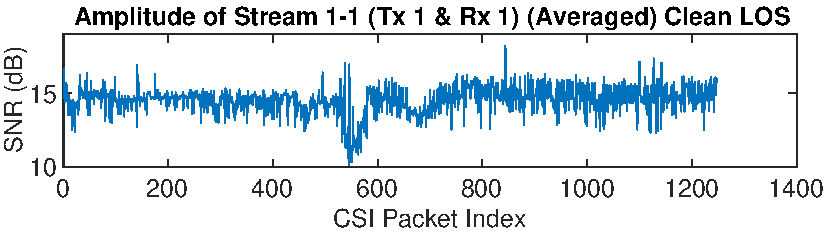
\includegraphics[scale = 0.5]{Figures/cleanLOSForAmplitude.pdf} }\\
\multicolumn{2}{c}{(c) Clean LOS from Tx-Rx}
\end{tabular}
\caption{CSI amplitude with with person falling, standing and then being absent (Clean LOS)}
\label{fig:diffamplitudes}%
\end{figure}
I carried out a number of tests using the averaged CSI amplitude as shown in Fig. 4.5. Mobile and immobile activities obtain different CSI amplitude variance with time. It is clear in (a) that something has occurred but this "fall" could also be confused with the fluctuation in (c) caused by the small disturbance closer to the receiver with nobody in the environment. It is hard to differentiate and recognise patterns between each of the situations. 
\subsection{CSI Phase}
I have noticed that CSI phase is more granular indication of a fall in an environment. I plotted the phase difference, as noted in PhaseU \citep{PhaseU}, below:
\begin{figure}[H]
    \centering
    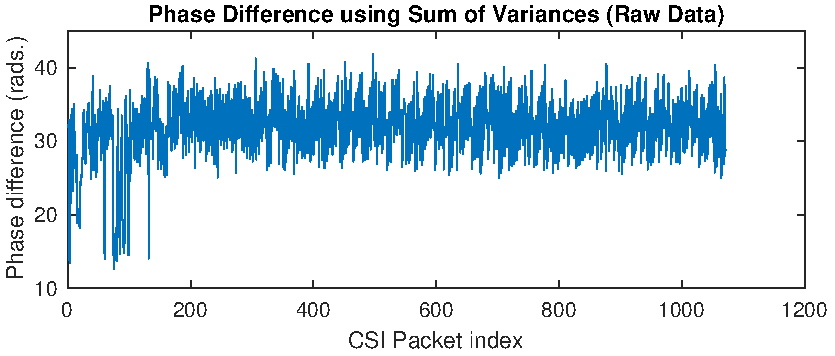
\includegraphics[scale=0.75]{Figures/uncleanPhaseFallCLASSROOM.pdf}
    \caption{Phase difference containing phase offsets and outliers}
    \label{fig:uncleanPhaseDiff}
\end{figure}
This plot above contains the unknown phase offset and timing offset as alluded to in Eqn. \ref{eqn:3.3} \& \ref{eqn:3.4}. No recognisable patterns in the data are noticeable. Using Eqn. \ref{eqn:3.5}, I can obtain a cleaner plot:
\begin{figure}[H]
    \centering
    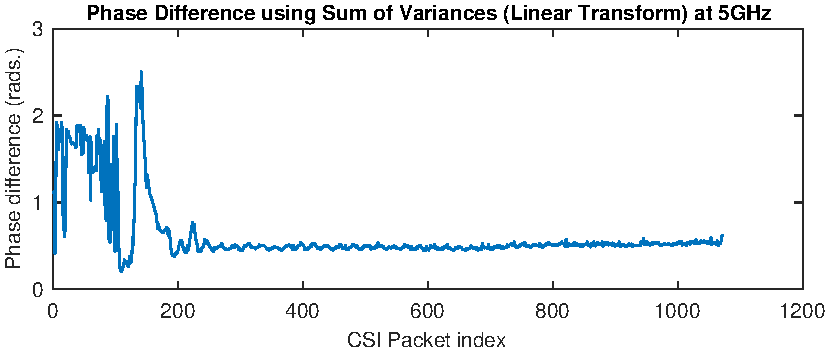
\includegraphics[scale=0.75]{Figures/cleanPhaseFallCLASSROOM.pdf}
    \caption{Phase difference from Fig. 4.7 after applying linear transform in Eqn. \ref{eqn:3.5}.}
    \label{fig:cleanerPhaseDiff}
\end{figure}
This plot has all phase offsets and outliers removed. The data is now interpretable in the time domain and human activities can be noticed. 
\subsection{Phase Difference \& Amplitude for Fall Detection}
Clearly, I have demonstrated the phase difference is a much more granular indicator of a human activity in an environment. I tested this using a "walking-fall" as shown below:
\begin{figure}[H]
    \centering
    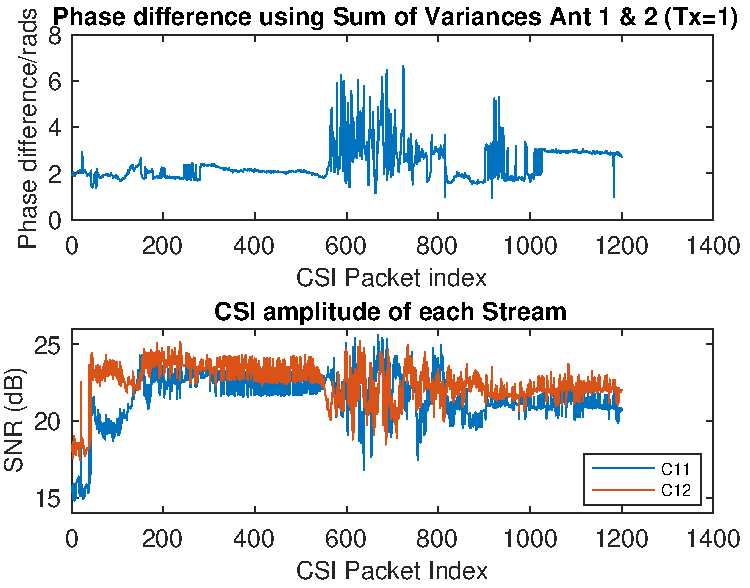
\includegraphics[scale=0.75]{Figures/subplotFall.pdf}
    \caption{CSI amplitude and transformed phase difference for 4m environment between Tx and Rx with a person walking into the environment, falling and standing up again. }
    \label{fig:finalPlot}
\end{figure}
Both the amplitude and phase difference experience a sudden disturbance on start up. This is a combination of the rate selection algorithm of the Archer C6 router adjusting and the test subject walking close to the receiver creating a multipath environment. The fall occurring just before the 600th packet creates a very large disturbance in the phase difference. The CSI amplitude suffers a disturbance also. However, the amplitude's response to the fall is very similar to the disturbance caused by the person walking between the 200th and 400th packet. The amplitude can be used for activity detection as in WiFall but isn't clear enough for fall detection. The phase difference clearly shows where the fall finished, save for a few oscillations. It is a much more sensitive indicator and the transformed phase is much less noisy than the amplitude. In a more complex MIMO-OFDM system, the phase difference resolution will improve due to the introduction of more antennas into the system and thus, performance for LOS/NLOS environments will greatly improve.